%%%%%%%%%%%%%%%%%%%%%%%%%%%%%%%%%%%%%%%%%
% Short Sectioned Assignment
% LaTeX Template
% Version 1.0 (5/5/12)
%
% This template has been downloaded from:
% http://www.LaTeXTemplates.com
%
% Original author:
% Frits Wenneker (http://www.howtotex.com)
%
% License:
% CC BY-NC-SA 3.0 (http://creativecommons.org/licenses/by-nc-sa/3.0/)
%
%%%%%%%%%%%%%%%%%%%%%%%%%%%%%%%%%%%%%%%%%

%----------------------------------------------------------------------------------------
%	PACKAGES AND OTHER DOCUMENT CONFIGURATIONS
%----------------------------------------------------------------------------------------

\documentclass[paper=a4, fontsize=11pt]{scrartcl} % A4 paper and 11pt font size

\usepackage[T1]{fontenc} % Use 8-bit encoding that has 256 glyphs
\usepackage{fourier} % Use the Adobe Utopia font for the document - comment this line to return to the LaTeX default
\usepackage[english]{babel} % English language/hyphenation
\usepackage{amsmath,amsfonts,amsthm} % Math packages

\usepackage{lipsum} % Used for inserting dummy 'Lorem ipsum' text into the template

\usepackage{sectsty} % Allows customizing section commands
\allsectionsfont{\centering \normalfont\scshape} % Make all sections centered, the default font and small caps

\usepackage{fancyhdr} % Custom headers and footers
\pagestyle{fancyplain} % Makes all pages in the document conform to the custom headers and footers
\fancyhead{} % No page header - if you want one, create it in the same way as the footers below
\fancyfoot[L]{} % Empty left footer
\fancyfoot[C]{} % Empty center footer
\fancyfoot[R]{\thepage} % Page numbering for right footer
\renewcommand{\headrulewidth}{0pt} % Remove header underlines
\renewcommand{\footrulewidth}{0pt} % Remove footer underlines
\setlength{\headheight}{13.6pt} % Customize the height of the header

\numberwithin{equation}{section} % Number equations within sections (i.e. 1.1, 1.2, 2.1, 2.2 instead of 1, 2, 3, 4)
\numberwithin{figure}{section} % Number figures within sections (i.e. 1.1, 1.2, 2.1, 2.2 instead of 1, 2, 3, 4)
\numberwithin{table}{section} % Number tables within sections (i.e. 1.1, 1.2, 2.1, 2.2 instead of 1, 2, 3, 4)

%\setlength\parindent{5pt} % Removes all indentation from paragraphs - comment this line for an assignment with lots of text

%----------------------------------------------------------------------------------------
%			ADDED PACKAGES, ETC.
%----------------------------------------------------------------------------------------
\usepackage{setspace} % Allows for double spacing, etc.
\usepackage{hyperref} % links within document
\hypersetup{
    colorlinks=true,
    linkcolor=blue,
    filecolor=magenta,      
    urlcolor=cyan,
}

\usepackage{graphicx}% allows figures
\graphicspath{ {./images/} } 
\usepackage[margin=1in]{geometry}
\usepackage{bm} % allows bold

\DeclareMathOperator{\EX}{\mathbb{E}}% expected value
 
%----------------------------------------------------------------------------------------
%				GLOSSARY
%----------------------------------------------------------------------------------------
% Type these commands at the command line after editing glossary:
% pdflatex summary
% makeglossaries summary
% pdflatex summary

\usepackage{glossaries}
\makeglossaries
\loadglsentries{glossary}
\glsaddall % makes sure all definitions are in glossary even if they aren't mentioned in text

%----------------------------------------------------------------------------------------
%	TITLE SECTION
%----------------------------------------------------------------------------------------

\newcommand{\horrule}[1]{\rule{\linewidth}{#1}} % Create horizontal rule command with 1 argument of height

\title{	
\normalfont \normalsize 
\horrule{0.5pt} \\[0.4cm] % Thin top horizontal rule
\huge Data Science Toolkit \\ % The assignment title
\horrule{2pt} \\[0.5cm] % Thick bottom horizontal rule
}

\author{Matt Goodwin} % Your name

\date{\normalsize\today} % Today's date or a custom date
\onehalfspacing


%----------------------------------------------------------------------------------------
%	BEGIN DOCUMENT
%----------------------------------------------------------------------------------------

\begin{document}

% Print the title
\maketitle 

% Table of Contents
\tableofcontents
\newpage

%----------------------------------------------------------------------------------------
%	SECTION 1
%----------------------------------------------------------------------------------------

\section{Statistical Modeling}
\subsection{Overview and Theory}

When discussing modeling it is important to keep in mind that ``all models are wrong but some are useful'' (attributed to George Box). The world is extremely complex and it can be impossible to create a model that perfectly approximates the underlying mechanisms that make our world turn.

There are different approaches to modeling depending on the discipline you come from, but personally I like the idea of the function approximation approach suggested by applied math and statistics. Taking this approach allows is to use probability theory combined with decision theory and to be able to visualize these concepts in a euclidean geometric space.

Bishop has a really nice overview of some of these concepts. The starting point I think for modeling starts with independent variable $X$ (which could be a vector, see \hyperref[sec:notation]{notation} section) and dependent variable $Y$. We want to know:

\begin{enumerate}
\item The nature of the relationship between the variables (inference). 
\item Given an independent variable, determine the dependent variable (prediction).
\end{enumerate}

Using probability we can completely summarize the relationship and the uncertainty between the two variables with the joint distribution $P(X,Y)$. We use probability because in problems we are interested in we generally cannot come to a completely deterministic relationship between the independent and dependent variables. This is in part because the number of independent variables needed to perfectly determine the dependent variable is potentially infinite. 

For example, imagine we wanted to predict the number of ice cream cones we sell on a particular day. Some variables such as the time of year or location of the ice cream store may provide us enough information to make a pretty good prediction or to understand the relationship between the independent and dependent variables fairly well. But to perfectly predict the number of ice cream cones we would need to know everything from the state of the road conditions, to whether or not a family from out of state decided to take a vacation. Since this is impossible we acknowledge variability and error in our estimates using probability.

This has been a sticking point for me of how to understand this, but I think the key is to remember that the moment we use only a subset of all the possible features we would need for a perfectly deterministic relationship, then we must introduce uncertainty. We cannot say for certain that knowing today is July 1 will lead to high ice-cream sales, but we can say the probability is higher than January 1st. When I have a training sample $(x_1, y_1), (x_2, y_2), ... (x_n, y_n)$ I treat this as the truth (which it is) but I need to remember that this is coming from a distribution. I guess in that sense $P(X,Y)$ is a model itself, something we are forced to use because we don't know all the features needed for a deterministic relationship.

As mentioned, we may want to perform inference, meaning understanding what $P(X,Y)$ looks like from a sample.  This can give us an understanding of how the variables are related (it can also allow us to do prediction but that is another step). In many practical applications we want to be able to predict $Y$ given $X$. This is where decision theory comes into play.

Decision theory is designed to help us make the optimal decision given inputs. Bishop gives a nice overview that I try and summarize in my own words below.

Lets approach this by treating the dependent variable $Y$ as a categorical variable taking on values 0 or 1. For simplicity assume $X$ is a single continuous variable. We then have for $P(X,Y)$ a three-dimensional distribution where $P(Y|X)$ is a probability mass function. When making a decision called the \emph{decision step} we formulate some rule that dived the input space into regions where if an instance falls into that region (based of $X$) it is predicted to be a 0 or 1. We want to minimize our mistakes as much as possible so we aren't assigning an instance to 0 when it should really be 1. The probability of mistake can be written as:

\begin{equation}
P(mistake) = P(X\in R_1, 0) + P(X\in R_0, 1)
\end{equation}
where $R_1$ is the region where an instance is assigned a 1 and $R_0$ is the region where an instance is assigned a 0.

Back to our example. Instead of ice cream sales, treat $Y$ as a categorical variable where 1 is a good ice cream day and 0 is bad.  If X = July 1st is in $R_1$ we decide to assign it a 1, based on our decision rule. However, even though our model $P(X,Y)$ says that the probability of a high selling day is high in this region, there is a still a chance that it is a low selling day because again, we are using a probability distribution since we don't have all of the features we need. The probability of it being a low selling day for all $X$ in $R_1$ is $P(X\in R_1, 0)$, which is a mistake.

 \begin{figure}[t] \label{fig:bishop_optimal_distributions}
\caption{Plot from Bishop showing visually the optimal decision boundary}
\centering
 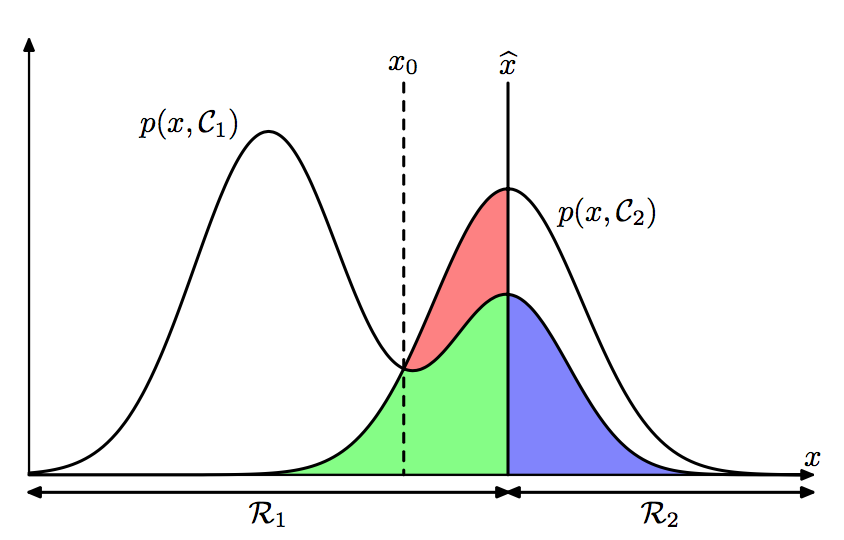
\includegraphics[scale=.7]{bishop_optimal_distributions.png}
 \end{figure}
 
We want to minimize our mistakes as much as possible so we choose regions where $P(X\in R_1, 0) + P(X\in R_0, 1)$ is as small as possible. To me it is easier to see by thinking of the probability of being correct which we want to maximize. The optimal decision boundary therefore is the location that creates $R_1$ and $R_0$ such that $P(X\in R_1, 1) >  P(X\in R_1, 0)$ everywhere in $R_1$ and $P(X\in R_0, 0) >  P(X\in R_0, 1)$ everywhere in $R_0$. If the decision boundary were shifted either way then we would loose out on area under the distribution of being correct. If we look at figure \ref{fig:bishop_optimal_distributions} then imagine the probability of being correct as all of the two humped distribution all colored in. If we went with $\hat{x}$ then we loose out on the red region for being correct.

 We can use the product rule to write:
 
 \begin{equation}
 \begin{split}
 P(X\in R_1, 1) >  P(X\in R_1, 0)  & =  P(1|X\in R_1) P(X \in R_1) > P(0|X\in R_1) P(X \in R_1) \\
 & =  P(1|X\in R_1) > P(0|X\in R_1) 
 \end{split}
 \end{equation}
 So we should chose the higher conditional probability for each region as well. TODO: I think this is the Bayes optimal decision rule?
 
 



Maybe one of the most simplest models to start with is the additive error model. This is given simply as:

\begin{equation}
Y = f(X) + \epsilon
\end{equation}


\begin{equation}
L(Y - \hat{f}(X)) = (Y - \hat{f}(X))^2
\EX[L(Y - \hat{f}(X))]
\end{equation}


\subsection{Bias-Variance Tradeoff}

The bias-variance tradeoff refers to two sources of error when evaluating models - the bias and the variance. There is also a third source of error which we call the ``irreducible error''. 

As explained in \href{https://towardsdatascience.com/mse-and-bias-variance-decomposition-77449dd2ff55}{this} article, there is a slight confusion in data science between decomposing the error for an \gls{estimator}, and decomposing the error for a model or a predictor. The decomposition is really about the same but there are some key insights to be aware of. The decomposition below is for a predictor. The decomposition for an estimator can be found in various books and other resources such as Casella/Berger. 

First of all bias is defined as:

\begin{equation}
Bias()
\end{equation}


\subsection{Generalized Linear Models}

There are three main components that make up the Generalized Linear Model (GLM):

\begin{enumerate}
\item Random component - assume the response variable comes from a probability distribution
\begin{equation}
Y_i \sim f(\mu_i)
\end{equation}
where $\mu_i = E(Y_i)$ and $f$ is a probability distribution.
\item Link component - connects the random component to the systematic component
\begin{equation}
g(\mu_i)=\eta_i
\end{equation}
\item Systematic component - this is the linear part
\begin{equation}
\eta_i = x_i^\prime \beta
\end{equation}

\end{enumerate}


\subsubsection{Logistic Regression}

Using the component concepts outlined above, for logistic regression we have:

\begin{enumerate}
\item Random component: $Y_i \sim f(\pi_i)$ where $f$ is the Bernoulli distribution (since $Y$ will be a binary variable when using logistic regression). $E(Y_i) = \pi_i $ which is the probability that $Y_i$ is 1.
\item Link component: this is the logit function which is defined as:
\begin{equation}
\text{logit}(\pi_i) = \log \left(\frac{\pi_i}{1-\pi_i} \right) = \eta_i
\end{equation}
\item Systematic component: tying this all together we have:
\begin{equation}
\log \left(\frac{\pi_i}{1-\pi_i}\right) = x_i^\prime \beta
\end{equation}
\end{enumerate}

Assumptions:
\begin{enumerate}
\item Linearity in log-odds
\item Independence of $Y_i|x_i$ and $Y_j|x_j$
\item Bernoulli response variable
\end{enumerate}

For interpretation we can say that with a one unit increase in $X_1$ for example, then the log odds of a success goes up by $\beta_1$. We can also use the multiplicative odds where a one unit increase in $X_1$ leads to a $e^{\beta_1}$ multiplicative change in odds on average.

The probability can be calculated by:
\begin{equation}
\begin{split}
\log \left(\frac{\pi_i}{1-\pi_1} \right) & = \beta_0 + x_i \beta_1 \\
\frac{\pi_i}{1-\pi_i} &= e^{\beta_0 + x_i \beta_1} \\
\pi_i &= e^{\beta_0 + x_i \beta_1} - e^{\beta_0 + x_i \beta_1} \pi_i \\
\pi_i &= \frac{e^{\beta_0 + x_i \beta_1}}{1+e^{\beta_0 + x_i \beta_1}}
\end{split}
\end{equation}


\subsection{Boosting}

The concept of boosting has lead to some of the most powerful algorithms in machine learning. Boosting falls under a general class of algorithms known as ensembles (bagging would be another example of ensemble algorithms where we run separate models and then aggregate at the end by averaging for example). The general concept is that we run a weak learner on the original data, calculate the errors, run a new model on the errors, combine with the first weak learner, and repeat until some stopping criteria (that avoids overfitting).

\subsubsection{Adaboost}


\section{Terms and Notation}

\subsection{Variable notiation}
\label{sec:notation}

Below explains notation used commonly when setting-up machine learning models. Note that all vectors are assumed to be column vectors. To help understand the notation I use the example of predicting the sales of ice cream cones. 
\vspace{2mm}

\begin{itemize}
\item $X$ - represents an input variable. Even though input variable implies a single variable this could also be a vector. If we wanted to access a single variable from the input vector then we use notation $X_j$. So for example $X$ could include variables that describe the temperature ($X_{j}$), time or year ($X_{j+1}$), etc. 
\item $Y$ - represents a \emph{quantitative} output variable. This could be the sales of ice cream cones in dollars.
\item $G$ - represents a \emph{qualitative} output variable. This could be if we sale over 50 ice cream cones for example (yes or no). 
\item $x_i$ - represents an observed value of the variable $X$. Again this could be a vector. So to get the observed scalar value of the temperature for example we would write $x_{ij}$. 
\item $\bm{X}$ - matrix typically with dimensions $Nxp$. 
\item $\bm{x_j}$ -  in general vectors are not bold unless the distinction is being made that this is the vector of all observation on $X_j$. So $\bm{x_j}$ is of length $N$ and $x_i$ is of length $p$.
\end{itemize}


\section{Basic Statistical Concepts}

\subsection{Inference}

Inference is referring to using data to figure out the underlying properties of a population (which in turn allows us to understand the relationship between variables). I've been thinking of inference as referring to the process to understand the relationship between variables in a linear regression, but I think this is too narrow of a view. For example, if we look at using a t-test to compare two samples what we are really doing is using the data to estimate what the two distributions are that the data comes from and then determine if that is reasonable or not. TODO: How do the various techniques in statistics fit in with this idea of finding the parameters of the underlying data?


\clearpage
\printglossaries

\end{document}